\documentclass[10pt]{article}
\usepackage[spanish]{babel}
\usepackage[utf8]{inputenc}
\usepackage{graphicx} 
\title{M\'etodos abiertos, Newton-Raphson}
\author{R\'omulo Walter Condori Bustincio}
\date{}
\begin{document}
\maketitle
\begin{enumerate}
\item para el primer an\'alisis, se considera la siguiente funci\'on $$x^3 + 3x^2 - 5$$, cuya gr\'afica es la siguiente:
\begin{center}
 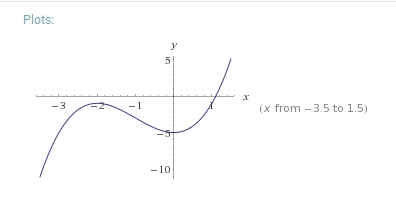
\includegraphics[scale=0.8]{./grafica1.jpg}
 % grafica1.jpg: 0x0 pixel, 300dpi, 0.00x0.00 cm, bb=
\end{center}
\begin{itemize}
 \item Con el algoritmo que se le proporciona la derivada, se genera la siguiente tabla:
 Con un total de 6 de 100000 iteraciones permitidas, se obtuvo la siguiente tabla:
\begin{center}
\begin{tabular}{|c|c|c|}
\hline
Iteraci\'on&$r$&$f(r)$\\
\hline
0&7&485\\
1&4.43386&141.143\\
2&2.78462&39.8545\\
3&1.78751&10.297\\
4&1.28053&2.01906\\
5&1.12032&0.171496\\
6&1.10397&0.00169663\\
\hline
\end{tabular}
\end{center}
Donde el valor de $r$ aproximado es 1.10397 con un error relativo de: 0.000165041

 \item Con el algoritmo que utiliza la derivada aproximada, se genera la siguiente tabla:
 Con un total de 6 de 100000 iteraciones permitidas, se obtuvo la siguiente tabla:
\begin{center}
\begin{tabular}{|c|c|c|}
\hline
Iteraci\'on&$r$&$f(r)$\\
\hline
0&7&485\\
1&4.43386&141.143\\
2&2.78462&39.8545\\
3&1.78751&10.297\\
4&1.28053&2.01906\\
5&1.12032&0.171496\\
6&1.10397&0.00169665\\
\hline
\end{tabular}
\end{center}
Donde el valor de $r$ aproximado es 1.10397 con un error relativo de: 0.000165043
\end{itemize}
\item para el segundo an\'alisis, se considera la siguiente funci\'on $$x-e^{\cos(5x-1)}\tan^{-1}(x^3+2x-4)$$,
 cuya gr\'afica es la siguiente:
\begin{center}
 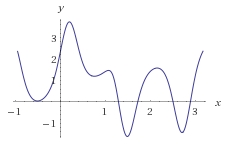
\includegraphics[scale=0.9]{./grafica2.jpg}
 % grafica1.jpg: 0x0 pixel, 300dpi, 0.00x0.00 cm, bb=
\end{center}
\begin{itemize}
 \item Con el algoritmo que se le proporciona la derivada, se genera la siguiente tabla:
 \begin{center}
\begin{tabular}{|c|c|c|}
\hline
Iteraci\'on&$r$&$f(r)$\\
\hline
0&7&6.32887\\
1&4.71925&4.03309\\
2&8.94667&4.81002\\
3&10.1207&6.66561\\
4&10.8138&10.2026\\
5&5.7459&5.08017\\
6&3.88096&0.0465492\\
7&3.88736&0.00143627\\
\hline
\end{tabular}
\end{center}
Donde el valor de $r$ aproximado es 3.88736 con un error relativo de: 0.000210459
 \item Con el algoritmo que utiliza la derivada aproximada, se genera la siguiente tabla:
 Con un total de 29 de 100000 iteraciones permitidas, se obtuvo la siguiente tabla:
\begin{center}
\begin{tabular}{|c|c|c|}
\hline
Iteraci\'on&$r$&$f(r)$\\
\hline
0&7&6.32887\\
1&4.71926&4.03308\\
2&8.94564&4.8143\\
3&10.0937&6.93612\\
4&10.7675&10.0913\\
5&7.19275&6.56693\\
6&34.9122&34.1442\\
7&55.2008&53.44\\
8&62.0994&60.6055\\
9&54.9359&54.3196\\
10&666.832&666.253\\
11&109.627&105.85\\
12&99.1041&97.9132\\
13&119.841&117.793\\
14&109.007&108.341\\
15&259.924&258.888\\
16&329.696&327.615\\
17&299.869&299.281\\
18&108.459&105.626\\
19&99.9675&99.2477\\
20&69.4382&65.8852\\
21&63.5889&62.9735\\
22&33.2199&31.8879\\
23&29.0068&25.1922\\
24&32.2376&31.6595\\
25&3.33502&2.7661\\
26&0.786295&1.19813\\
27&-3.70939&-0.363054\\
28&-3.67841&-0.0181715\\
29&-3.67667&-8.27564e-05\\
\hline
\end{tabular}
\end{center}
Donde el valor de $r$ aproximado es -3.67667 con un error relativo de: 8.01425e-06
\end{itemize}

\item Los fragmentos del c\'odigo utilizado son:
\begin{itemize}
 \item C\'odigo con derivada exacta proporcionada por el usuario:
 \begin{center}
 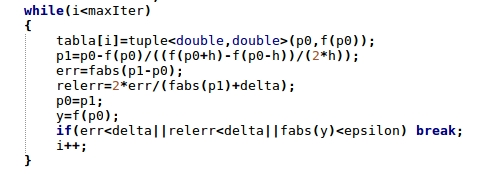
\includegraphics[scale=0.8]{./code1.jpg}
 % grafica1.jpg: 0x0 pixel, 300dpi, 0.00x0.00 cm, bb=
\end{center}
\item C\'odigo con derivada aproximada:
\begin{center}
 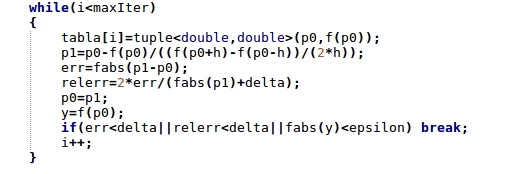
\includegraphics[scale=0.8]{./code2.jpg}
 % grafica1.jpg: 0x0 pixel, 300dpi, 0.00x0.00 cm, bb=
\end{center}
\end{itemize}


\end{enumerate}
\end{document}
